\graphicspath{{./figures/}}
\date{}
\begin{document}
\begin{frame}
    \titlepage
\end{frame}


\makeatletter
\newenvironment<>{btHighlight}[1][]
{\begin{onlyenv}#2\begingroup\tikzset{bt@Highlight@par/.style={#1}}\begin{lrbox}{\@tempboxa}}
{\end{lrbox}\bt@HL@box[bt@Highlight@par]{\@tempboxa}\endgroup\end{onlyenv}}

\newcommand<>\btHL[1][]{%
  \only#2{\begin{btHighlight}[#1]\bgroup\aftergroup\bt@HL@endenv}%
}
\def\bt@HL@endenv{%
  \end{btHighlight}%   
  \egroup %
}
\tikzset{
    btHLbox/.style={
        fill=red!30,outer sep=0pt,inner xsep=1pt, inner ysep=0pt, rounded corners=3pt
    },
}
\newcommand{\bt@HL@box}[2][]{%
  \tikz[#1]{%
    \pgfpathrectangle{\pgfpoint{1pt}{0pt}}{\pgfpoint{\wd #2}{\ht #2}}%
    \pgfusepath{use as bounding box}%
    \node[text width={},draw=none,anchor=base west, btHLbox, minimum height=\ht\strutbox+1pt,#1]{\raisebox{1pt}{\strut}\strut\usebox{#2}};
  }%
}

\lst@CCPutMacro
    \lst@ProcessOther {"2A}{%
      \lst@ttfamily 
         {\raisebox{2pt}{*}}% used with ttfamily
         {\raisebox{2pt}{*}}}% used with other fonts
    \@empty\z@\@empty

\lstdefinelanguage
   [x8664gas]{Assembler}     % add a "x64" dialect of Assembler
   [x86masm]{Assembler} % based on the "x86masm" dialect
   % with these extra keywords:
   {morekeywords={CDQE,CQO,CMPSQ,CMPXCHG16B,JRCXZ,LODSQ,MOVSXD,%
                  POPFQ,PUSHFQ,SCASQ,STOSQ,IRETQ,RDTSCP,SWAPGS,.TEXT,.STRING,.ASCIZ,%
                  BEQ,LW,SW,LB,SB,ADDIU,J,BEQZ,BNEZ,BNE,%
                  MOVUPD,MULPD,MOVSD,MULSD,%
                  SHLADD,MOV,CMP.LT,TBIT.NZ,BR.RET.SPTK.MANY,%
                  ADDQ,POPQ,PUSHQ,RRMOVQ,MRMOVQ,RMMOVQ,IRMOVQ,%
                  <-,LL,SC,ADDI,ADDL,VMOVDQA,ADDQ,CMPL,JB,JBE,MOVL,CLTQ,%
                  MOVW,PUSHW,MOV,ADD,SUB,INT,PUSH,MOV,ADD,REP,MOVSB,%
                  TESTQ,CMPQ,MOVL,MOVQ,ADDQ,JMPQ,XORQ,%
                  LEAQ,LEAL,LEA,RETQ,RET,POPL,POPW,PUSHL,PUSHW,%
                  LEAW,%
                  SUBQ,SYSCALL,.ASCII,CALLQ,MOVSLQ,JMP,ANDQ,SHRQ,MOVB,INCQ,TESTL,XORL,%
                  SHRL,LEAL,SARL,SUBL,IMULL,IMULQ,MOVDQU,PADDD,XORL,%
                  MOVZBL,MOVZB,SHRB,SRAL,SHRL,ANDL,%
                  CMOVNS,SRAL,SRAQ,MOVZBW,MOVZBQ,%
                  PADDW,PADDQ,MODUPS,MOVAPD,%
                  MOVL,RET,.GLOBL,%
		  PAUSE,LFENCE,JMP,%
                  },
    deletekeywords={eax,ebx,sp,si,cx,di,ds,cs,es,fs,dx,ax,bx,al,esi,ebp,ecx,rip,eip,edx,edi,rdi,esp},
    deletekeywords=[2]{size},
    alsoletter={\%},
    alsoother={()},
    emphstyle={\color{violet!50!black}},
    emph={\%rax,\%rbx,\%rcx,\%rdx,\%r8,\%r9,\%r10,\%r11,\%r12,\%r13,\%r14,\%r15,\%eax,\%ebx,\%sp,\%si,\%cx,\%di,\%ds,\%cs,\%es,\%fs,\%dx,\%ax,\%bx,\%al,\%esi,\%ebp,\%ecx,\%rip,\%eip,\%edx,\%edi,\%rdi,\%esp,\%rsp},
    %moreemph={eax,ebx,sp,si,cx,di,ds,cs,es,fs,dx,ax,bx,al,esi,ebp,ecx,rip,eip,edx,edi,rdi,esp},
    morecomment=[l]{\#},
    morecomment=[l]{\/\/},
    morecomment=[s]{/*}{*/},
    sensitive=false,
    keepspaces=true} % et

\lstalias[]{myasm}[x8664gas]{Assembler}

\lstdefinelanguage{JavaScript}{
  keywords={typeof, new, true, false, catch, function, return, null, catch, switch, var, if, in, while, do, else, case, break},
  ndkeywords={class, export, boolean, throw, implements, import, this},
  sensitive=false,
  comment=[l]{//},
  morecomment=[s]{/*}{*/},
  morestring=[b]',
  morestring=[b]"
}

\newcommand{\keywordstyle}{\sourcecodeprolight\bfseries\color{blue!30!black}}
\newcommand{\stringstyle}{\color{blue!20!black}\ttfamily}

\lstset{
    language=C,
    basicstyle=\sourcecodepro\EmptyMapping,
    escapechar=`,
    keywordstyle=\keywordstyle\EmptyMapping,
    identifierstyle=\sourcecodepro\EmptyMapping,
    numberstyle=\small\color{black!70},
    commentstyle=\color{red!60!black}\ttfamily\itshape,
    stringstyle=\color{blue!20!black}\ttfamily,
    ndkeywordstyle=\bfseries\color{blue!30!black},
    upquote=true,
}



\lstdefinestyle{medium}{
    basicstyle=\sourcecodepro\EmptyMapping\fontsize{12}{13}\selectfont,
    keywordstyle=\sourcecodepro\EmptyMapping\fontsize{12}{13}\selectfont\keywordstyle,
}

\lstdefinestyle{small}{
    basicstyle=\sourcecodepro\EmptyMapping\small,
    keywordstyle=\sourcecodepro\EmptyMapping\small\keywordstyle,
}

\lstdefinestyle{smaller}{
    basicstyle=\sourcecodepro\EmptyMapping\fontsize{11}{12}\selectfont,
    keywordstyle=\sourcecodepro\EmptyMapping\fontsize{11}{12}\selectfont\keywordstyle,
}

\lstdefinestyle{size105}{
    basicstyle=\sourcecodepro\EmptyMapping\fontsize{10.5}{11.5}\selectfont,
    keywordstyle=\sourcecodepro\EmptyMapping\fontsize{10.5}{11.5}\selectfont\keywordstyle,
}

\lstdefinestyle{size10}{
    basicstyle=\sourcecodepro\EmptyMapping\fontsize{10}{11}\selectfont,
    keywordstyle=\sourcecodepro\EmptyMapping\fontsize{10}{11}\selectfont\keywordstyle,
}

\lstdefinestyle{size9}{
    basicstyle=\sourcecodepro\EmptyMapping\fontsize{9}{10}\selectfont,
    keywordstyle=\sourcecodepro\EmptyMapping\fontsize{9}{10}\selectfont\keywordstyle,
}
\lstdefinestyle{size8}{
    basicstyle=\sourcecodepro\EmptyMapping\fontsize{8}{9}\selectfont,
    keywordstyle=\sourcecodepro\EmptyMapping\fontsize{8}{9}\selectfont\keywordstyle,
}



\lstdefinestyle{script}{
    basicstyle=\sourcecodepro\EmptyMapping\scriptsize,
    keywordstyle=\sourcecodepro\EmptyMapping\scriptsize\bfseries,
}




\usetikzlibrary{arrows.meta,calc,matrix,positioning}

\section{aside on ASLR}
\subsection{actual stack location}

\begin{frame}[fragile,label=stackLoc1]{stack location?}
\begin{Verbatim}[fontsize=\fontsize{9}{10}\selectfont]
$ cat stackloc.c
#include <stdio.h>
int main(void) {
    int x;
    printf("%p\n", &x);
}
$ ./stackloc.exe
0x7ffe8859d964
$ ./stackloc.exe
0x7ffd4e26ac04
$ ./stackloc.exe
0x7ffc190af0c4
\end{Verbatim}
\end{frame}



\subsection{without ASLR}

\begin{frame}[fragile,label=stackLoc2]{disabling ASLR}
\vspace{-.5cm}
\begin{Verbatim}[fontsize=\fontsize{9}{10}\selectfont]
$ cat stackloc.c
#include <stdio.h>
int main(void) {
    int x;
    printf("%p\n", &x);
}
$ setarch x86_64 -vRL bash
Switching on ADDR_NO_RANDOMIZE.
Switching on ADDR_COMPAT_LAYOUT.
$ ./stackloc.exe 
0x7fffffffde2c
$ ./stackloc.exe 
0x7fffffffde2c
$ ./stackloc.exe 
0x7fffffffde2c
\end{Verbatim}
\end{frame}


\subsection{ASLR preview}
\begin{frame}{address space layout randomization (ASLR)}
    \begin{itemize}
    \item vary the location of things in memory
    \item including the stack
    \item designed to make exploiting memory errors harder
    \item will talk more about later
    \end{itemize}
\end{frame}


\subsection{still varies without ASLR?}

\begin{frame}[fragile,label=stackLoc3a]{stack location? (take 2a)}
\begin{Verbatim}[fontsize=\fontsize{9}{10}\selectfont]
$ ./stackloc.exe 
0x7fffffffde2c
$ gdb ./stackloc.exe
...
(gdb) run
Starting program: .../stackloc.exe 
0x7fffffffdd9c
[Inferior 1 (process 833005) exited normally]
\end{Verbatim}
\end{frame}


\begin{frame}[fragile,label=stackLoc3b]{stack location? (take 2b)}
\begin{Verbatim}[fontsize=\fontsize{9}{10}\selectfont]
$ ./stackloc.exe 
0x7fffffffde2c
$ ./stackloc.exe 
0x7fffffffde2c
$ ./stackloc.exe test
0x7fffffffde1c
$ ./stackloc.exe test
0x7fffffffde1c
$ $(pwd)/stackloc.exe
0x7fffffffdd8c
$ $(pwd)/stackloc.exe
0x7fffffffdd8c
\end{Verbatim}
\end{frame}


\section{mitigations, generally}
\usetikzlibrary{positioning,shapes.callouts}
\begin{frame}{exploit mitigations}
    \begin{itemize}
    \item idea: turn vulnerablity to something less bad
    \item e.g. crash instead of machine code execution
    \vspace{.5cm}
    \item many of these targetted at buffer overflows
    \end{itemize}
\end{frame}

\begin{frame}{mitigation agenda}
    \begin{itemize}
        \item we will look briefly at one mitigation --- stack canaries
        \item then look at exploits that don't care about it
        \item then look at more flexible mitigations
        \item then look at more flexible exploits
    \end{itemize}
\end{frame}

\begin{frame}<1>[label=mitigationPrios]{mitigation priorities}
    \begin{itemize}
    \item \myemph<2>{effective?}\tikzmark{effective} does it actually stop the attacker?
    \item fast? how much does it hurt performance?
    \item generic? does it require a recompile? rewriting software?
    \end{itemize}

    \begin{tikzpicture}[overlay,remember picture]
        \begin{visibleenv}<2>
        \node[my callout=effective,anchor=center,align=center] at (current page.center) {
            recurring theme: stop stack smashing, \\ but not other buffer overflows
        };
        \end{visibleenv}
    \end{tikzpicture}
\end{frame}


\section{mitigating stack smashing}

\begin{frame}<1-2>[label=stopSmashing]{stopping stack smashing?}
    \begin{itemize}
    \item how can you stop stack smashing?
    \vspace{.5cm}
    \item<2-> stop overrun --- bounds-checking
    \item<2-> \myemph<3>{stop return to attacker code}
    \item<2-> stop execution of attacker code
    \end{itemize}
\end{frame}




\section{stack canaries}
\subsection{in code}
\usetikzlibrary{decorations.pathreplacing,decorations.pathmorphing}

\begin{frame}<1>[fragile,label=reCanary]{compiler generated code}
\lstset{
    language=myasm,
    style=smaller,
    moredelim={**[is][\btHL<2|handout:0>]{~2~}{~end~}},
    moredelim={**[is][\btHL<3|handout:0>]{~3~}{~end~}},
}
\vspace{-.25cm}
\begin{lstlisting}
    pushq %rbx
    sub $0x20,%rsp
/* copy value from thread-local storage */
    mov $0x28,%ebx
    mov %fs:(%rbx),%rax
/* onto the stack */
    mov %rax,0x18(%rsp)
/* clear register holding value */
    ~2~xor %eax, %eax~end~
    ...
    ...
/* copy value back from stack */
    mov 0x18(%rsp),%rax
/* xor to compare */
    ~2~xor %fs:(%rbx),%rax~end~
/* if result non-zero, do not return */
    jne call_stack_chk_fail
    ret
call_stack_chk_fail:
    call __stack_chk_fail
\end{lstlisting}
\begin{tikzpicture}[overlay,remember picture]
\begin{pgfonlayer}{fg}
    \coordinate (stack tl) at ([xshift=-4cm,yshift=-1cm]current page.north east);
    \coordinate (stack tr) at ([xshift=-.5cm,yshift=-1cm]current page.north east);
    \draw[very thick] (stack tl) -- ++(0, -6) coordinate (stack bl);
    \draw[very thick] (stack tr) -- ++(0, -6) coordinate (stack br);
    \draw[very thick,decorate,decoration={zigzag}] (stack tl) -- (stack tr);
    \draw[very thick,decorate,decoration={zigzag}] (stack bl) -- (stack br);
\end{pgfonlayer}
\path[draw,thick,fill=yellow!20] (stack tl) ++(0cm, -1cm) coordinate (ra tl) rectangle ++(3.5, -.5) coordinate (ra br)
    node [midway] {return address};
\coordinate (ra bl) at (ra tl |- ra br);
\path[draw,thick,fill=red!20] (ra bl) rectangle ++(3.5, -.5) coordinate (can br)
    node [midway] {stack canary};
\coordinate (can bl) at (ra tl |- can br);
\path[draw,thick,fill=green!20,align=center,font=\small] (can bl) rectangle ++(3.5, -2) 
    node [midway] {function's \\ arrays \\ and other \\ temporaries};
\begin{pgfonlayer}{fg}
    \begin{visibleenv}<2>
    \node[fill=white,draw=red,very thick,anchor=east,align=center] at ([xshift=-1cm]current page.east) {
        trying to avoid info disclosure: \\
        get canary value out of \%rax \\
        as soon as possible
    };
    \end{visibleenv}
\end{pgfonlayer}
\end{tikzpicture}
\end{frame}



\subsection{general operation}
\usetikzlibrary{arrows.meta}

\begin{frame}[fragile,label=returnToStackCanaryPic]{stack canary}
\begin{tikzpicture}
% FIXME:
\tikzset{
    stackBox/.style={very thick},
    onStack/.style={thick},
    xscale=1.3,
}
\draw[stackBox] (0, 0) rectangle (10, -6);
\draw[thick,-Latex] (10.25,-5) -- (10.25, -1) node [midway, below, sloped] {increasing addresses};
\node[at={(5, 0.1)},anchor=south] { highest address (stack started here)};
\node[at={(5, -6.1)},anchor=north] { lowest address (stack grows here)};

\draw[onStack] (0, -.25) rectangle (10, -1.25) node[midway,align=center,font=\small] (stackAddr)
     {return address for {\tt vulnerable}: \\
     \only<1>{\fontsize{10}{11}\selectfont\tt\color{black}37 fd 40 00  00 00 00 00 (0x40fd37)}
     \only<2>{\fontsize{10}{11}\selectfont\tt\bfseries\color{red}70 fd ff ff  ff ff 00 00 (0x7fff ffff fd70)}};
\draw[onStack,fill=black!20] (0, -1.25) rectangle (10, -1.75) node[midway,align=center,font=\small] {canary: \only<1>{\tt b1 ab bd e8 31 15 df 31}\only<2>{\color{red}{\tt ?? ?? ?? ?? ?? ?? ??}}};
\draw[onStack,fill=black!20] (0, -1.75) rectangle (10, -2.25) node[midway,align=center,font=\small] {unused space (12 bytes)};
\draw[onStack,fill=blue!20] (0, -2.25) rectangle (10, -5.25) node[midway,align=center,font=\small] {buffer (100 bytes)};

\draw[onStack] (0, -5.25) rectangle (10, -6) node[midway,align=center,font=\small] {return address for {\tt scanf}};

\begin{visibleenv}<2>
\draw[-Latex,red,ultra thick] ([yshift=2.5mm]stackAddr.south east) -- ++(.25cm,0cm) |- (0.25, -5);
\node[anchor=south west,red] at (0.25, -4.75) {
    machine code for the attacker to run
};
\end{visibleenv}

\end{tikzpicture}
\end{frame}



\subsection{requirements and how they can fail to be met}

\begin{frame}<1>[label=stackCanHopes]{stack canary hopes}
    \begin{itemize}
    \item \myemph<2>{overwrite return address $\implies$ overwrite canary}
    \item \myemph<3>{canary is secret}
    \end{itemize}
\end{frame}


 % FIXME: repeat slide with highlites

\subsection{how glibc generates canaries}

\begin{frame}{good choices of canary}
\begin{itemize}
\item \myemph{random} --- guessing should not be practical
    \begin{itemize}
    \item not always --- sometimes static or only $2^{15}$ possible
    \end{itemize}
\item GNU libc: canary contains:
\vspace{.5cm}
    \item leading {\tt \textbackslash 0} (string terminator)
        \begin{itemize}
        \item {\tt printf \%s} won't print it
        \item copying a C-style string won't write it
        \end{itemize}
    \item a newline
        \begin{itemize}
        \item read line functions can't input it
        \end{itemize}
    \item {\tt \textbackslash xFF}
        \begin{itemize}
        \item hard to input?
        \end{itemize}
\end{itemize}
\end{frame}


\subsection{GCC and canaries}

\begin{frame}{stack canaries implementation}
    \begin{itemize}
    \item ``StackGuard'' --- 1998 paper proposing strategy
    \item GCC: command-line options
        \begin{itemize}
        \item {\tt -fstack-protector} 
        \item {\tt -fstack-protector-strong} 
        \item {\tt -fstack-protector-all}
        \item one of these often default
        \item three differ in how many functions are `protected'
        \end{itemize}
    \item Microsoft C/C++ compiler: {\tt /GS}
        \begin{itemize}
        \item on by default
        \end{itemize}
    \end{itemize}
\end{frame}




\subsection{canary costs}

\begin{frame}{stack canary overheads}
    \begin{itemize}
    \item less than 1\% runtime if added to ``risky'' functions
        \begin{itemize}
        \item functions with character arrays, etc.
        \end{itemize}
    \item large overhead if added to all functions
        \begin{itemize}
        \item StackGuard paper: 5--20\%?
        \end{itemize}
    \item similar space overheads
    \vspace{.5cm}
    \item (for typical applications)
        \begin{itemize}
        \item could be much worse: tons of `risky' function calls
        \end{itemize}
    \end{itemize}
\end{frame}




\subsection{overall pros/cons}

\begin{frame}{stack canaries pro/con}
    \begin{itemize}
        \item pro: no change to calling convention
        \item pro: recompile only --- no extra work
        \item con: can't protect existing executable/library files (without recompile)
        \item con: \myemph<2>{doesn't protect against many ways of exploiting buffer overflows}
        \item con: \myemph<3>{vulnerable to information leaks}
    \end{itemize}
\end{frame}




\subsection{stack canary summary}

\begin{frame}{stack canary summary}
    \begin{itemize}
    \item stack canary --- simplest of many \myemph{mitigations}
    \item key idea: detect corruption of return address
    \item assumption: if return address changed, so is adjacent token
    \item assumption: attacker can't learn true value of token
        \begin{itemize}
        \item often possible with memory bug
        \end{itemize}
    \vspace{.5cm}
    \item later: workarounds to break these assumptions
    \end{itemize}
\end{frame}




\subsection{noncontiguous overwrites}
\againframe<2>{stackCanHopes}
\usetikzlibrary{decorations.pathreplacing,decorations.pathmorphing}

\begin{frame}[fragile,label=stackNonContig]{non-contiguous overwrites}
\begin{lstlisting}[style=small]
void vulnerable() {
  int scores[8]; bool done = false;
  while (!done) {
    cout << "Edit which score? (0 to 7) ";
    int i;
    cin >> i;
    /* Oops!
       sizeof(scores) is 8 * sizeof(int) */
    if (i < 0 || i >= sizeof(scores))
      continue;
    cout << "Set to what value?" << endl;
    cin >> scores[i];
    ...
  }
  ...
}
\end{lstlisting}
\begin{tikzpicture}[overlay,remember picture,y=1.25cm]
\begin{pgfonlayer}{fg}
\coordinate (stack tl) at ([xshift=-4cm,yshift=-1cm]current page.north east);
\coordinate (stack tr) at ([xshift=-.5cm,yshift=-1cm]current page.north east);
\draw[very thick] (stack tl) -- ++(0, -6) coordinate (stack bl);
\draw[very thick] (stack tr) -- ++(0, -6) coordinate (stack br);
\draw[very thick,decorate,decoration={zigzag}] (stack tl) -- (stack tr);
\draw[very thick,decorate,decoration={zigzag}] (stack bl) -- (stack br);
\end{pgfonlayer}
\path[draw,thick,fill=yellow!20] (stack tl) ++(0cm, -1cm) coordinate (ra tl) rectangle ++(3.5, -.5) coordinate (ra br)
    node [midway] {return address};
\coordinate (ra bl) at (ra tl |- ra br);
\path[draw,thick,fill=red!20] (ra bl) rectangle ++(3.5, -.5) coordinate (can br)
    node [midway] {stack canary};
\coordinate (can bl) at (ra tl |- can br);
\foreach \x/\idx in {0/7, 1/6, 2/5, 3/4, 4/3, 5/2, 6/1, 7/0} {
    \path[draw,thick,fill=green!20,align=center,font=\small] (can bl) ++ (0, -\x * 0.25)
        rectangle ++(3.5, -0.25)  node[midway,font=\tt\fontsize{9}{10}\selectfont]{scores[\idx]};
}
\path[fill=violet!30,opacity=0.5] (can bl) ++ (0, -8 * 0.25) rectangle ++(3.5, -1.5) 
    node[midway,font=\fontsize{9}{10}\selectfont,align=center] {stack grows here for \\ calls to cin/cout \\ methods};
\end{tikzpicture}
\end{frame}


%FIXME: polls entry for exercise
\usetikzlibrary{decorations.pathreplacing,decorations.pathmorphing}

\begin{frame}[fragile,label=stackNonContigEx]{exercise: non-contiguous overwrites}
\begin{lstlisting}[style=small]
void vulnerable() {
  int scores[8]; bool done = false;
  while (!done) {
    cout << "Edit which score? (0 to 7) ";
    int i;
    cin >> i;
    /* Oops!
       sizeof(scores) is 4 * sizeof(int) */
    if (i < 0 || i >= sizeof(scores))
      continue;
    cout << "Set to what value?" << endl;
    cin >> scores[i];
    ...
  }
  ...
}
\end{lstlisting}
\begin{tikzpicture}[overlay,remember picture,y=1.25cm]
\begin{pgfonlayer}{fg}
\coordinate (stack tl) at ([xshift=-4cm,yshift=-1cm]current page.north east);
\coordinate (stack tr) at ([xshift=-.5cm,yshift=-1cm]current page.north east);
\draw[very thick] (stack tl) -- ++(0, -6) coordinate (stack bl);
\draw[very thick] (stack tr) -- ++(0, -6) coordinate (stack br);
\draw[very thick,decorate,decoration={zigzag}] (stack tl) -- (stack tr);
\draw[very thick,decorate,decoration={zigzag}] (stack bl) -- (stack br);
\end{pgfonlayer}
\path[draw,thick,fill=yellow!20] (stack tl) ++(0cm, -1cm) coordinate (ra tl) rectangle ++(3.5, -.5) coordinate (ra br)
    node [midway] {return address};
\coordinate (ra bl) at (ra tl |- ra br);
\path[draw,thick,fill=red!20] (ra bl) rectangle ++(3.5, -.5) coordinate (can br)
    node [midway] {stack canary};
\coordinate (can bl) at (ra tl |- can br);
\foreach \x/\idx in {0/7, 1/6, 2/5, 3/4, 4/3, 5/2, 6/1, 7/0} {
    \path[draw,thick,fill=green!20,align=center,font=\small] (can bl) ++ (0, -\x * 0.25)
        rectangle ++(3.5, -0.25)  node[midway,font=\tt\fontsize{9}{10}\selectfont]{scores[\idx] (4 byte)};
}
\path[fill=violet!30,opacity=0.5] (can bl) ++ (0, -8 * 0.25) rectangle ++(3.5, -1.5) 
    node[midway,font=\fontsize{9}{10}\selectfont,align=center] {stack grows here for \\ calls to cin/cout \\ methods};
\node[draw=red,anchor=south,very thick,align=center,fill=white] at ([xshift=-2cm,yshift=.25cm]current page.south) {
    exercise: to set return address to 0x123456789, \\
    set what scores to what values?
};
\end{tikzpicture}
\end{frame}



\subsection{information disclosure}
\againframe<3>{stackCanHopes}
\subsubsection{examples}
\begin{frame}[fragile,label=infoDisc1a]{information disclosure (1a)}
\lstset{
    language=C++,
    style=small
}
\begin{lstlisting}
string command;
void vulnerable() {
    int value;
    for (;;) {
        cin >> command;
        if (command == "set") {
            cin >> value;
        } else if (command == "get") {
            cout << value << endl;
        } else if ...
    }
}
\end{lstlisting}
\begin{itemize}
\item ``get'' command: can read \myemph{uninitialized value}
\item example: when I compiled this, \texttt{value} was stored on the stack
\end{itemize}
\end{frame}

\begin{frame}[fragile,label=infoDisc1b]{information disclosure (1b)}
\lstset{
    language=C++,
    style=small
}
\begin{lstlisting}
void vulnerable() {
    int value;
    ...
        } else if (command == "get") {
            cout << value << endl;
        }
    ...
}

void leak() {
    int secrets[] = { 
        12345678, 23456789, 34567890,
        45678901, 56789012, 67890123,
    };  
    cout << (void*) secrets << endl;
    do_something_with(secrets);
}

int main() {leak(); vulnerable();}
\end{lstlisting}
\begin{tikzpicture}[overlay,remember picture]
\node[draw,very thick,anchor=north east,align=left] at ([xshift=-.25cm,yshift=-.25cm]current page.north east) {
running this program \\
(input in bold): \\
\tt \textbf{get} \\
\tt 67890123
};
\end{tikzpicture}
\end{frame}

\begin{frame}[fragile,label=infoDisc2]{information disclosure (2)}
\lstset{
    language=C,
    style=small
}
\begin{lstlisting}
void process() {
    char buffer[8] = "\0\0\0\0\0\0\0\0";
    char c = ' ';
    for (int i = 0; c != '\n' && i < 8; ++i) {
        c = getchar();
        buffer[i] = c;
    }
    printf("You input %s\n", buffer);
}
\end{lstlisting}
\begin{itemize}
\item input \verb|aaaaaaaa|
\item output \verb|You input aaaaaaaa|{\it (whatever was on stack)}
\end{itemize}
\end{frame}

\begin{frame}[fragile,label=infoDisc3]{information disclosure (3)}
\lstset{
    language=C,
    style=small,
}
\begin{lstlisting}
struct foo {
    char buffer[8];
    long *numbers;
};

void process(struct foo* thing) {
    ...
    scanf("%s", thing->buffer);
    ...
    printf("first number: %ld\n", thing->numbers[0]);
}
\end{lstlisting}
\begin{itemize}
\item input: {\tt aaaaaaaa}\textit{(address of canary)}
    \begin{itemize}
    \item address on stack \textit{or} where canary is read from in thread-local storage
    \end{itemize}
\end{itemize}
\end{frame}



\subsubsection{exercise}
\begin{frame}{recall: ASLR}
    \begin{itemize}
    \item easlier mentioned ASLR (address space layout randomization)
    \item for stack: choose secret starting address for stack
    \vspace{.5cm}
    \item info disclosure bugs are a big problem for this!
    \end{itemize}
\end{frame}

\begin{frame}[fragile,label=infoDiscEx]{exercise}
\begin{tikzpicture}
\node (first) {
\begin{lstlisting}[language=C,style=smaller]
struct point {
    int x, y, z;
};
\end{lstlisting};
};
\node[anchor=north west] at (first.north east) {
\begin{lstlisting}[language=C,style=smaller]
struct point *p;
...
    if (command == "get") { 
        /* 'p' could be uninitialized */
        printf("%d,%d,%d\n", p->x, p->y, p->z);
    } ...
...
\end{lstlisting}
};
\end{tikzpicture}
\vspace{-.25cm}
\begin{itemize}
\item Which initial value for \texttt{p} (``left over'' from prior use of register, etc.) would be most useful for figuring out the address of the stack pointer?
\begin{itemize}
\item A. \texttt{p} is an invalid pointer and accessing it will crash the program
\item B. \texttt{p} points to space on the stack that is currently unallocated, but last contained an input buffer
\item C. \texttt{p} points to a struct allocated on the heap
\item D. \texttt{p} points to space on the stack that currently holds a return address
\item E. \texttt{p} points to space on the stack that is currently unallocated, but last contained a pointer to the last used byte of an input buffer on the stack
\end{itemize}
\end{itemize}
\end{frame}


\subsubsection{avoiding?}
\againframe<2>{reCanary}

% FIXME: exercise: using info disclosure bug?


\section{memory protection}
\subsection{generally}
\usetikzlibrary{arrows.meta,shapes.multipart,patterns,positioning}
\begin{frame}[fragile,label=vm]{recall(?): virtual memory}
\begin{itemize}
\item illuision of \myemph{dedicated memory}
\end{itemize}
\begin{tikzpicture}
\tikzset{
    every node/.style={font=\small},
}
\node[align=center] (progAAddr) {Program A \\ addresses};
\node[below=1cm of progAAddr,align=center] (progBAddr) {Program B \\ addresses};
\node[draw, right=1cm of progAAddr,align=center] (translationA) { mapping \\ (set by OS) };
\node[draw, right=1cm of progBAddr,align=center] (translationB) { mapping \\ (set by OS) };
\node[draw,rectangle split, rectangle split parts=6, anchor=north west,label={north:real memory}] (mem) at ([xshift=1cm]translationA.north east) {
    \nodepart{one}
    Program A code 
    \nodepart{two}
    Program B code
    \nodepart{three}
    Program A data
    \nodepart{four}
    Program B data
    \nodepart{five}
    OS data
    \nodepart{six}
    \ldots
};
\draw[-Latex,green,thick] (progAAddr) -- (translationA) (translationA.east) -- (mem.one west);
\draw[-Latex,green,thick] (translationA.east) -- (mem.three west);
\draw[-Latex,blue,thick] (progBAddr) -- (translationB) (translationB.east) -- (mem.two west);
\draw[-Latex,blue,thick] (translationB.east) -- (mem.four west);
\node[thick,red,draw,anchor=north west] (error) at ([yshift=-.5cm]mem.south west) {trigger error};
\draw[-Latex,green,thick] (translationA.east) -- (error.west);
\draw[-Latex,blue,thick] (translationB.east) -- (error.west);
\draw[-Latex,green,ultra thick,dotted] (translationA.east) -- (mem.five west);
\draw[-Latex,blue,ultra thick,dotted] (translationB.east) -- (mem.five west);
\draw[-Latex,ultra thick,dotted] ([xshift=-3cm,yshift=-.5cm]translationB.south) -- ([xshift=-2cm,yshift=-.5cm]translationB.south)
    node[right] {= kernel-mode only};
\end{tikzpicture}
\end{frame}



\subsection{page-level permissions}
\usetikzlibrary{matrix}
\begin{frame}<1>[label=mappingList]{the mapping (set by OS)}
\begin{tikzpicture}
\tikzset{
    dot/.style={draw=none}
}
\matrix[tight matrix,nodes={minimum height=.525cm,text width=3cm,font=\small\tt},
    row 1/.style={nodes={font=\bfseries\small\normalfont}},
    column 1/.style={nodes={draw=none,text width=6cm}},
    column 2/.style={nodes={text width=1cm}},
    column 3/.style={nodes={text width=1cm}},
    column 4/.style={nodes={alt=<2>{opacity=1.0,red}{opacity=0.0},text width=1cm}},
] {
program address range \& read? \& write? \& exec? \& real address\\
0x0000 --- 0x0FFF \& no \& no \& no \& --- \\
0x1000 --- 0x1FFF \& no \& no \& no \& --- \\
|[dot]| \ldots \\
0x40 0000 --- 0x40 0FFF \& yes \& no \& yes \& 0x... \\
0x40 1000 --- 0x40 1FFF \& yes \& no \& yes \& 0x... \\
0x40 2000 --- 0x40 2FFF \& yes \& no \& yes \& 0x... \\
|[dot]| \ldots \\
0x60 0000 --- 0x60 0FFF \& yes \& yes \& no\& 0x... \\
0x60 1000 --- 0x60 1FFF \& yes \& yes \& no\& 0x... \\
|[dot]| \ldots \\
|[font=\scriptsize]| 0x7FFF FF00 0000 --- 0x7FFF FF00 0FFF \& yes \& yes \& no\& 0x... \\
|[font=\scriptsize]| 0x7FFF FF00 1000 --- 0x7FFF FF00 1FFF \& yes \& yes \& no\& 0x... \\
|[dot]| \ldots \\
};
\end{tikzpicture}
\end{frame}

\begin{frame}{Virtual Memory}
    \begin{itemize}
    \item modern \myemph{hardware-supported} memory protection mechanism
    \item via \myemph{table}: OS decides \myemph{what memory program sees}
        \begin{itemize}
        \item whether it's read-only or not
        \end{itemize}
    \item granularity of \myemph{pages} --- typically 4KB
    \vspace{.5cm}
    \item not in table --- segfault (OS gets control)
    \end{itemize}
\end{frame}




\subsection{guard pages / replacing stack canaries?}
\usetikzlibrary{arrows.meta,shapes.multipart,patterns}

\tikzset{
    stackBox/.style={very thick},
    onStack/.style={thick},
    frameOne/.style={fill=blue!15},
    frameTwo/.style={fill=red!15},
    markLine/.style={blue!50!black},
    markLineB/.style={red!90!black},
    hiLine/.style={red!90!black},
}

\begin{frame}{malloc/new guard pages}
\begin{tikzpicture}
    \draw[thick,-Latex] (-0.25,-5) -- (-0.25, -1) node [midway, above, sloped] {increasing addresses};
    \node[anchor=south] at (3, 0) {the heap};
    \draw[stackBox] (0, 0) rectangle (6, -6);
    \draw[onStack,fill=blue!20] (0, -2) rectangle (6, -3.5)
        node[midway,align=center] {\texttt{malloc(6000)} \\ (or \texttt{new char[6000]}) };
    \draw[onStack,pattern=north west lines,pattern color=red] (0, -1) rectangle (6, -2)
        node[midway,fill=white] {guard page};
    \draw[onStack,pattern=north west lines,pattern color=red] (0, -4) rectangle (6, -5)
        node[midway,fill=white] {guard page};
    \draw[onStack,fill=black!20] (0, -3.5) rectangle (6, -4)
        node[midway] {unused space};
\end{tikzpicture}
\end{frame}

\begin{frame}{guard pages}
    \begin{itemize}
    \item deliberate holes
    \item accessing --- segfualt
    \item call to OS to allocate (not very fast)
    \item likely to `waste' memory
        \begin{itemize}
        \item guard around object? minimum 4KB object
        \end{itemize}
    \end{itemize}
\end{frame}

\begin{frame}{guard pages for malloc/new}
    \begin{itemize}
    \item can implement malloc/new by placing guard pages around allocations
        \begin{itemize}
        \item commonly done by real malloc/new's for \myemph{large allocations}
        \end{itemize}
    \item problem: minimum actual allocation 4KB
    \item problem: substantially slower
    \item example: ``Electric Fence'' allocator for Linux (early 1990s)
    \end{itemize}
\end{frame}


\begin{frame}[fragile,label=stackGuard]{stack canary alternative}
\begin{tikzpicture}
\draw[stackBox] (0, 0) rectangle (6, -6);
\draw[thick,-Latex] (-.25,-5) -- (-.25, -1) node [midway, above, sloped] {increasing addresses};
\node[at={(4, 0.1)},anchor=south] { highest address (stack started here)};
\node[at={(4, -6.1)},anchor=north] { lowest address (stack grows here)};

\draw[onStack] (0, -.25) rectangle (6, -1.25) node[midway,align=center,font=\small] (stackAddr)
     {return address for {\tt vulnerable}: \\
     {\fontsize{10}{11}\selectfont\tt\color{black}0x40fd37}
     };
    \draw[onStack,pattern=north west lines,pattern color=red] (0, -1.25) rectangle (6, -3.25) node[midway,align=center,font=\small,fill=white] {``guard page'' \\ minimum 4KB};
\draw[onStack,fill=blue!20] (0, -3.25) rectangle (6, -4.25) node[midway,align=center,font=\small] {buffer};
\begin{visibleenv}<2->
\draw[black,Latex-] (6.1, -1.25) -- ++(.5cm, 0cm) node[right,font=\small\tt] {0x7FFFF 2000};
\draw[black,Latex-] (6.1, -3.25) -- ++(.5cm, 0cm) node[right,font=\small\tt] {0x7FFFF 1000};

\matrix[tight matrix,overlay,
    column 1/.style={nodes={text width=2.25cm,minimum height=1cm,font=\fontsize{9}{10}\selectfont\tt}},
    column 2/.style={nodes={minimum height=1cm}},
    column 3/.style={nodes={minimum height=1cm}},
    ] at (12.4, -2) {
        address \& read \& write \\
    0x7FFFF2000- 0x7FFFF2FFF \& yes \& yes \\
    0x7FFFF1000- 0x7FFFF1FFF \& no \& no \\
    0x7FFFF0000- 0x7FFFF0FFF \& yes \& yes \\
};
\end{visibleenv};

\end{tikzpicture}
\end{frame}

\begin{frame}[fragile,label=stackGuardB]{stack canary alternative 2}
\begin{tikzpicture}
\draw[stackBox] (0, 0) rectangle (6, -6);
\draw[thick,-Latex] (-.25,-5) -- (-.25, -1) node [midway, above, sloped] {increasing addresses};
\node[at={(4, 0.1)},anchor=south] { highest address (stack started here)};
\node[at={(4, -6.1)},anchor=north] { lowest address (stack grows here)};

\draw[onStack] (0, -.25) rectangle (6, -1.25) node[midway,align=center,font=\small] (stackAddr)
     {return address for {\tt vulnerable}: \\
     {\fontsize{10}{11}\selectfont\tt\color{black}0x40fd37}
     };
\draw[onStack,pattern=north west lines,pattern color=black!50] (0, -1.25) rectangle (6, -2.25) node[midway,align=center,font=\small,fill=white] {unused space};
\draw[onStack,fill=blue!20] (0, -2.25) rectangle (6, -4.25) node[midway,align=center,font=\small] {buffer};
\begin{visibleenv}<2->
\draw[black,Latex-] (6.1, -.25) -- ++(.5cm, 0cm) node[right,font=\small\tt] {0x7FFFF 2000};
\draw[black,Latex-] (6.1, -2.25) -- ++(.5cm, 0cm) node[right,font=\small\tt] {0x7FFFF 1000};

\matrix[tight matrix,
    column 1/.style={nodes={text width=2.25cm,minimum height=1cm,font=\fontsize{9}{10}\selectfont\tt}},
    column 2/.style={nodes={minimum height=1cm}},
    column 3/.style={nodes={minimum height=1cm}},
    ] at (12.3, -1) {
        address \& read \& write\\
    0x7FFFF2000- 0x7FFFF2FFF \& yes \& yes \\
    0x7FFFF1000- 0x7FFFF1FFF \& yes \& \myemph<2>{no} \\
    0x7FFFF0000- 0x7FFFF0FFF \& yes \& yes \\
};
\end{visibleenv};

\end{tikzpicture}
\end{frame}



\subsection{exercise: guard page overhead}
\begin{frame}{exercise: guard page overhead}
    \begin{itemize}
    \item suppose heap allocations are:
        \begin{itemize}
        \item $100\,000$ objects of 100 bytes
        \item $1\,000$ objects of 1000 bytes
        \item $100$ objects of approx. 10000 bytes
        \end{itemize}
    \item total allocation of approx 12 000 KB
    \item assuming 4KB pages, estimate space overhead of using guard pages:
        \begin{itemize}
        \item for objects larger than 4096 bytes (1 page)
        \item for objects larger than 200 bytes
        \item for all objects
        \end{itemize}
    \end{itemize}
\end{frame}


\subsection{read-only pages}
\begin{frame}{recall: function pointer targets}
    \begin{itemize}
    \item wanted to overwrite special pointer:
    \vspace{.5cm}
    \item return addresses on stack
    \item function pointers on in local variables
    \item tables of function pointers used for inheritence
    \item global offset table
    \vspace{.5cm}
    \item last two: need to change infrequently
    \item idea: make read-only
    \end{itemize}
\end{frame}

\begin{frame}{RELRO}
    \begin{itemize}
        \item \textbf{REL}ocation \textbf{R}ead-\textbf{O}nly
        \item Linux option: make dynamic linker structures read-only after startup
        \item partial RELRO: everything but GOT pointers to library functions
            \begin{itemize}
            \item notably includes C++ virtual function tables
            \end{itemize}
        \item full RELRO: everything including those pointers
            \begin{itemize}
            \item requires disabling ``lazy'' linking
            \item (could do without disabling --- but slower (how much?) startup)
            \end{itemize}
        \item appears as ELF program header entry
    \end{itemize}
\end{frame}




\subsection{non-executable pages}
\begin{frame}{a thought on permissions}
    \begin{itemize}
    \item if we can set memory non-writeable
    \item how about non-executable?
    \vspace{.5cm}
    \item we never want to execute things on the stack anyways, right?
    \end{itemize}
\end{frame}


\begin{frame}[fragile,label=wxorx]{write XOR execute}
    \begin{itemize}
    \item many names:
    \begin{itemize}
        \item \verb|W^X| (write XOR execute)
        \item DEP (Data Execution Prevention)
        \item NX bit (No-eXecute) (hardware support)
        \item XD bit (eXecute Disable) (hardware support)
    \end{itemize}
    \item mark writeable memory as executable
    \item how will users insert their machine code?
        \begin{itemize}
        \item can only code in application + libraries
        \item a problem, right?
        \end{itemize}
    \end{itemize}
\end{frame}



\subsubsection{unfortunate history of HW/SW support}

\begin{frame}{hardware support for write XOR execute}
    \begin{itemize}
    \item everywhere today
    \item not historically common
    \item early x86: execute implied by read
    \item NX support added with x86-64 and around 2000 for x86-32
    \end{itemize}
\end{frame}

\begin{frame}{deliberate use of writeable code}
    \begin{itemize}
    \item ``just-in-time'' (JIT) compilers
        \begin{itemize}
        \item fast virtual machine/language implementations
        \end{itemize}
    \item some weird GCC features
    \item older ``signals'' on Linux
        \begin{itemize}
        \item OS wrote machine code on stack for program to run
        \end{itemize}
    \item couldn't even disable executable stacks without breaking applications
    \end{itemize}
\end{frame}



\subsubsection{if you can't write machine code}
\begin{frame}{why doesn't W xor X solve the problem?}
    \begin{itemize}
    \item W xor X is ``almost free'', keeps attacker from writing code?
    \item problem: useful machine code is in program already
        \begin{itemize}
        \item just need to find writable function pointer
        \end{itemize}
    \item saw special case: arc injection
        \begin{itemize}
        \item happened to find useful code in existing application/library
        \end{itemize}
    \item turns out: almost always useful code
    \end{itemize}
\end{frame}


\section{ASLR}
\subsection{what it is}

\begin{frame}{address space layout randomization (ASLR)}
    \begin{itemize}
    \item assume: addresses don't leak
    \item choose \myemph{random} addresses each time
        \begin{itemize}
        \item for \myemph{everything}, not just the stack
        \end{itemize}
    \item \myemph{enough possibilities} that attacker won't ``get lucky''
    \item should prevent exploits --- can't write GOT/shellcode location
    \end{itemize}
\end{frame}



\subsection{how much entropy}
\usetikzlibrary{calc,positioning,patterns,shapes.callouts}

\begin{frame}{Linux stack randomization (x86-64)}
\begin{itemize}
    \item 1. choose random number between \texttt{0} and \tikzmark{range}\myemph<2>{\texttt{0x3F FFFF}}
    \item 2. stack starts at \texttt{0x7FFF FFFF FFFF} - \textit{random number} $\times$ \texttt{0x1000}
        \begin{itemize}
        \item randomization disabled? \textit{random number} $= 0$
        \end{itemize}
\end{itemize}
\begin{tikzpicture}[overlay,remember picture]
\node[my callout=range] at ([yshift=-1cm]current page.center) {
    16 GB range!
};
\end{tikzpicture}
\end{frame}

\begin{frame}<1>[fragile,label=aslr64]{program memory (x86-64 Linux; ASLR)}
\begin{tikzpicture}[remember picture]
\tikzset{
    mylabel/.style={font=\ttfamily,align=center,append after command={([xshift=.1cm]\tikzlastnode.west) edge[ultra thick] ++(-.2cm,0cm)}},
    mybox/.style={draw,rectangle,minimum width=7cm,fill=white},
    myhigh/.style={draw,rectangle,line width=1mm, draw=blue!80!black,opacity=.3},
}
\node[mybox,minimum height=.5cm,inner ysep=0mm,pattern=north west lines,pattern color=black!50!white] (kernel) {Used by OS};
\begin{pgfonlayer}{bg}
    \node[right=1mm of kernel.north east,mylabel] (topLabel) {0xFFFF FFFF FFFF FFFF};
    \node[right=1mm of kernel.south east,mylabel] {0xFFFF 8000 0000 0000};
\end{pgfonlayer}
\node[mybox, minimum height=.5cm, below=.45cm of kernel] (stack) {Stack};
\begin{pgfonlayer}{bg}
    \node[right=1mm of stack.north east,mylabel] {\myemph<1>{$\pm$ 0x004 0000 0000}};
\end{pgfonlayer}
\node[mybox, minimum height=.5cm, below=0.5cm of stack] (heapB) {Dynamic/Non-fixed exe/Libraries (mmap)};
\begin{pgfonlayer}{bg}
    \node[right=1mm of heapB.north east,mylabel] (heapBLabel) {\myemph<1>{$\pm$ 0x100 0000 0000}};
    \node[below=0mm of heapBLabel,font=\small,inner sep=0mm] {(filled from top with ASLR)};
\end{pgfonlayer}
%\begin{pgfonlayer}{bg}
%    \node[right=1mm of heapB.south east,mylabel] (heapBLabel) {0x0000 2baa aaaa b000 \\ $\pm$ 0x100 0000 0000\*};
%\end{pgfonlayer}
\node[mybox, minimum height=.5cm, below=0.5cm of heapB] (heap) {Heap (brk/sbrk)};
\begin{pgfonlayer}{bg}
\node[right=1mm of heap.south east,mylabel] (heapBLabel) {\myemph<1>{$\pm$ 0x200 0000}};
\end{pgfonlayer}
\node[mybox, minimum height=.5cm, below=0.2mm of heap] (data) {Writable data if fixed exe addresses};
\begin{pgfonlayer}{bg}
\node[right=1mm of data.south east,mylabel] (bottomLabel) {\myemph<2-3>{0x0000 0000 0060 0000}*};
\node[below=0mm of bottomLabel,font=\small,inner sep=0mm] {(constants + 2MB alignment)};
\end{pgfonlayer}
\node[mybox, minimum height=.5cm, below=0.6cm of data] (sdata) {Code + Constants if fixed exe addresses};
\begin{pgfonlayer}{bg}
\node[right=1mm of sdata.south east,mylabel] (sbottomLabel) {\myemph<2-3>{0x0000 0000 0040 0000}};
\end{pgfonlayer}
\coordinate (memBottom) at ($(sdata.south east) + (0mm, -2mm)$);
\begin{pgfonlayer}{bg}
\draw[pattern=north west lines, pattern color=black!40!white] (kernel.north west) rectangle (memBottom);
\end{pgfonlayer}

\begin{visibleenv}<3>
    \begin{scope}[overlay]
    \node[draw=red,ultra thick,fill=white,anchor=center,
          inner sep=.5cm,font=\Large] at (current page.center) {
        why are these addresses fixed?
    }; 
    \end{scope}
\end{visibleenv}

\end{tikzpicture}
\end{frame}

\begin{frame}{program memory (x86-32 Linux; ASLR)}
\begin{tikzpicture}
\tikzset{
    mylabel/.style={font=\ttfamily,align=center,append after command={([xshift=.1cm]\tikzlastnode.west) edge[ultra thick] ++(-.2cm,0cm)}},
    mybox/.style={draw,rectangle,minimum width=7cm,fill=white},
    myhigh/.style={draw,rectangle,line width=1mm, draw=blue!80!black,opacity=.3},
}
\node[mybox,minimum height=.5cm,inner ysep=0mm,pattern=north west lines,pattern color=black!50!white] (kernel) {Used by OS};
\begin{pgfonlayer}{bg}
    \node[right=1mm of kernel.north east,mylabel] (topLabel) {0xFFFF FFFF};
    \node[right=1mm of kernel.south east,mylabel] {0xC000 0000};
\end{pgfonlayer}
\node[mybox, minimum height=.5cm, below=.5cm of kernel] (stack) {Stack};
\begin{pgfonlayer}{bg}
    \node[right=1mm of stack.north east,mylabel] {\myemph{$\pm$ 0x080 0000} (default)};
\end{pgfonlayer}
\node[mybox, minimum height=.5cm, below=0.5cm of stack] (heapB) {Dynamic/Libraries (mmap)};
\begin{pgfonlayer}{bg}
    \node[right=1mm of heapB.north east,mylabel] (heapBLabel) {\myemph{$\pm$ 0x008 0000} (default)};
\end{pgfonlayer}
%\begin{pgfonlayer}{bg}
%    \node[right=1mm of heapB.south east,mylabel] (heapBLabel) {0x0000 2baa aaaa b000 \\ $\pm$ 0x100 0000 0000\*};
%\end{pgfonlayer}
\node[mybox, minimum height=.5cm, below=0.5cm of heapB] (heap) {Heap (brk/sbrk)};
\begin{pgfonlayer}{bg}
\node[right=1mm of heap.south east,mylabel] (heapBLabel) {\myemph{$\pm$ 0x200 0000}};
\end{pgfonlayer}
\node[mybox, minimum height=.5cm, below=0.2mm of heap] (data) {Writable data};
\begin{pgfonlayer}{bg}
%\node[right=1mm of data.south east,mylabel] (bottomLabel) {0x0804 0000};
\end{pgfonlayer}
\node[mybox, minimum height=.5cm, below=0.6cm of data] (sdata) {Code + Constants if fixed exe addresses};
\begin{pgfonlayer}{bg}
\node[right=1mm of sdata.south east,mylabel] (bottomLabel) {0x0804 8000};
\end{pgfonlayer}
\coordinate (memBottom) at ($(sdata.south east) + (0mm, -2mm)$);
\begin{pgfonlayer}{bg}
\draw[pattern=north west lines, pattern color=black!40!white] (kernel.north west) rectangle (memBottom);
\end{pgfonlayer}
\end{tikzpicture}
\end{frame}

\begin{frame}{how much guessing?}
    \begin{itemize}
    \item gaps change by multiples of page (4K)
        \begin{itemize}
        \item lower 12 bits are \myemph{fixed}
        \end{itemize}
    \item 64-bit: \myemph{huge} ranges --- need millions of guesses
        \begin{itemize}
        \item about \myemph{30 randomized bits} in addresses
        \end{itemize}
    \item 32-bit: \myemph{smaller} ranges --- hundreds of guesses
        \begin{itemize}
        \item only about \myemph{8 randomized bits} in addresses
        \item why? only 4 GB to work with!
        \item can be configured higher --- but larger gaps
        \end{itemize}
    \end{itemize}
\end{frame}

\begin{frame}{why do we get multiple guesses?}
    \begin{itemize}
    \item why do we get multiple guesses?
    \vspace{.5cm}
    \item wrong guess might not crash
    \item wrong guess might not crash whole application
        \begin{itemize}
        \item e.g. server that uses multiple processes
        \end{itemize}
    \item local programs we can repeatedly run
    \item servers that are automatically restarted
    \end{itemize}
\end{frame}


\subsection{kept together: danger of leaks}

\begin{frame}[fragile,label=betweenSegments1]{dependencies between segments (1)}
\begin{lstlisting}[language={},style=smaller]
$ objdump -x foo.exe
...
LOAD off    0x0000000000000000 vaddr 0x0000000000000000 paddr 0x0000000000000000 align 2**12
     filesz 0x0000000000000620 memsz 0x0000000000000620 flags r--
LOAD off    0x0000000000001000 vaddr 0x0000000000001000 paddr 0x0000000000001000 align 2**12
     filesz 0x0000000000000205 memsz 0x0000000000000205 flags r-x
LOAD off    0x0000000000002000 vaddr 0x0000000000002000 paddr 0x0000000000002000 align 2**12
     filesz 0x0000000000000150 memsz 0x0000000000000150 flags r--
LOAD off    0x0000000000002db8 vaddr 0x0000000000003db8 paddr 0x0000000000003db8 align 2**12
     filesz 0x000000000000025c memsz 0x0000000000000260 flags rw-
\end{lstlisting}
\begin{itemize}
\item 4 seperately loaded segments: can we choose random addresses for each?
\end{itemize}
\end{frame}

\begin{frame}[fragile,label=betweenSegments2]{dependencies between segments (2)}
\begin{lstlisting}[language={},style=smaller,moredelim={**[is][\btHL<1->]{~2~}{~end~}}]
0000000000001050 <__printf_chk@plt>:
    1050:       f3 0f 1e fa             endbr64 
    1054:       f2 ff 25 75 2f 00 00    bnd jmpq *~2~0x2f75(%rip)        # 3fd0~end~ <__printf_chk@GLIBC_2.3.4>
    105b:       0f 1f 44 00 00          nopl   0x0(%rax,%rax,1)
\end{lstlisting}
\begin{itemize}
\item dependency from 2nd LOAD (0x1000-0x1205) to 4th LOAD (0x3db8-0x4018)
\item uses relative addressing rather than linker filling in address
\end{itemize}
\end{frame}

\begin{frame}[fragile,label=betweenSegments3]{dependencies between segments (3)}
\begin{lstlisting}[language={},style=smaller,moredelim={**[is][\btHL<1->]{~2~}{~end~}}]
0000000000001060 <main>:
    1060:       f3 0f 1e fa             endbr64 
    1064:       50                      push   %rax
    1065:       8b 15 a5 2f 00 00       mov    0x2fa5(%rip),%edx        # 4010 <global>
    106b:       48 8d 35 92 0f 00 00    lea    ~2~0xf92(%rip)~end~,%rsi        # 2004 <_IO_stdin_used+0x4>
    1072:       31 c0                   xor    %eax,%eax
    1074:       bf 01 00 00 00          mov    $0x1,%edi
    1079:       e8 d2 ff ff ff          callq  1050 <__printf_chk@plt>
\end{lstlisting}
\begin{itemize}
\item dependency from 2nd LOAD (0x1000-0x1205) to 3rd LOAD (0x2000-0x2150)
\item uses relative addressing rather than linker filling in address
\end{itemize}
\end{frame}

\begin{frame}[fragile,label=whyRipRelative]{why is this done?}
\begin{itemize}
\item Linux made a choice: \\
no editing code when loading programs, libraries\
\vspace{.5cm}
\item allows same code to be loaded in multiple processes
\end{itemize}
\end{frame}

\begin{frame}[fragile,label=noGuessing]{danger of leaking pointers}
    \begin{itemize}
        \item any stack pointer? know everything on the stack!
        \item any pointer within executable? know everything in the executable!
        \item any pointer to a particular library? know everything in library!
    \end{itemize}
\end{frame}



\subsection{exercise: using a leak}
\begin{frame}[fragile,label=useLeak1]{exericse: using a leak (1)}
\begin{lstlisting}[language=C++,style=small]
class Foo {
    virtual const char *bar() { ... }
};
...
Foo *f = new Foo;
printf("%s\n", f);
\end{lstlisting}
\begin{itemize}
\item Part 1: What address is most likely leaked by the above?
    \begin{itemize}
    \item A. the location of the Foo object allocated on the heap
    \item B. the location of the first entry in Foo's VTable"
    \item C. the location of the first instruction of Foo::Foo() (Foo's compiler-generated constructor)"
    \item D. the location of the stack pointer
    \end{itemize}
\end{itemize}
\end{frame}


\begin{frame}[fragile,label=useLeak2]{exercise: using a leak (2)}
\begin{lstlisting}[language=C++,style=script]
class Foo {
    virtual const char *bar() { ... }
};
...
Foo *f = new Foo;
char *p = new char[1024];
printf("%s\n", f);
\end{lstlisting}
\begin{itemize}
\item if leaked value was 0x822003 and in a debugger (with \textbf{different randomization}):
    \begin{itemize}
    \item stack pointer was 0x7ffff000
    \item Foo::bar's address was 0x400000
    \item f's address was 0x900000
    \item f's Vtable's address was 0x403000
    \item a ``gadget'' address from the main executable was 0x401034
    \item a ``gadget'' address from the C library was 0x2aaaa40034
    \item p's address was 0x901000
    \end{itemize}
\item which of the above can I compute based on the leak?
\end{itemize}
\end{frame}

\usetikzlibrary{arrows.meta,decorations.pathreplacing,decorations.pathmorphing}
\begin{frame}<1>[fragile,label=aslrTogether]{exes, libraries stay together}
\begin{tikzpicture}[remember picture]
\draw[thick,decorate,decoration={zigzag}] (0, 0) -- (6, 0);
\draw[thick] (0, 0) -- (0, -7);
\draw[thick] (6, 0) -- (6, -7);
\draw[thick,decorate,decoration={zigzag}] (0, -7) -- (6, -7);
\draw[thick,fill=yellow!10] (0, -1) rectangle ++(6, -0.8) node[midway] {foo.exe globals};
\draw[thick,fill=yellow!10] (0, -2) rectangle ++(6, -1.3) node[midway] {foo.exe code};
\draw[thick,fill=yellow!10] (0, -3.5) rectangle ++(6, -0.9) node[midway,align=center] {foo.exe constants \\ (likely has VTables)};
\draw[very thick,Latex-] (6, -4.4) -- ++ (1cm, 0cm) node[right] {this address can be randomized};
\draw[very thick,decorate,decoration={brace,mirror}] (6.1, -4.4) -- ++ (0cm, 3.4) node[midway,right,align=left] {
    must stay together \\
    code uses offset(\%rip) \\
    to access globals, constants
};
\end{tikzpicture}
\end{frame}



\subsection{alternate approach: Windows}

\begin{frame}{relocating: Windows}
    \begin{itemize}
        \item Windows will \myemph{edit code} to relocate
            \begin{itemize}
            \item not everything uses a GOT-like lookup table
            \end{itemize}
        \item typically one fixed location per program/library \textbf{per boot}
            \begin{itemize}
                \item same address used across all instances of program/library
                \item still allows sharing memory
            \end{itemize}
        \item fixup once per program/library per boot
            \begin{itemize}
                \item before ASLR: code could be pre-relocated
            \end{itemize}
        \item Windows + Visual Studio had `full' ASLR by default since 2010
    \end{itemize}
\end{frame}

\begin{frame}{Windows ASLR limitation}
    \begin{itemize}
        \item same address in all programs --- not very useful against local exploits
    \end{itemize}
\end{frame}



\subsection{making ASLR: removing hard-coded addresses}
\begin{frame}{PIC: Linux, OS X}
    \begin{itemize}
        \item Linux, OS X: position-independent code
        \item allows libraries code pages to be shared
        \item \ldots even if loaded at different addresses
        \vspace{.5cm}
        \item avoids per-boot randomization of Windows, but\ldots
    \end{itemize}
\end{frame}


\subsubsection{without absolute}
\begin{frame}[fragile,label=ex]{exercise: avoiding absolute addresses}
\lstset{
    language=myasm,
    style=smaller,
    escapeinside=~~,
}
\begin{tikzpicture}
\node[anchor=north east] (code) at (-1, 0) {
\begin{lstlisting}
foo:
	movl	$3, %eax
	cmpq	$5, %rdi
	ja	defaultCase
	jmp	*lookupTable(,%rdi,8)
returnOne:
        movl    $1, %eax
        ret
returnTwo:
        movl    $2, %eax
defaultCase:
        ret
\end{lstlisting}
};
\node[anchor=north west] (code2) at (-.5, 0) {
\begin{lstlisting}
lookupTable:
    .quad returnOne
    .quad returnTwo
    .quad returnOne
    .quad returnTwo
    .quad returnOne
    .quad returnOne
\end{lstlisting}
};
\end{tikzpicture}
\begin{itemize}
    \item exercise: rewrite this without absolute addresses
    \item but fast
\end{itemize}
\end{frame}



\subsection{changes with position-independent code}


\newcommand{\myemphTwo}[1]{\myemph<2>{#1}}%
\newcommand{\myemphThree}[1]{\myemph<3>{#1}}%
\newcommand{\myemphFour}[1]{\myemph<{#1}}%
\newcommand{\antiEmphThree}[1]{{\color<3>{blue}#1}}%
\newcommand{\antiEmphFour}[1]{{\color<4>{blue}#1}}%
\begin{frame}[fragile,label=PIEjtasm]{PIE jump-table}
\begin{tikzpicture}
\node[anchor=north east] (code) at (-1, 0) {
\lstset{
    language=myasm,
    style=smaller,
    escapeinside=~~,
}
\begin{lstlisting}
foo:
  movl	 $3, %eax
  cmpq	 $5, %rdi
  ja	 retDefault
  leaq	 ~\myemphTwo{jumpTable(\%rip)},~%rax
  movslq ~\myemphTwo{(\%rax,\%rdi,4)},~%rdx
  addq	 %rdx, %rax
  ~\myemphTwo{\bfseries jmp}~   ~\myemphTwo{*\%rax}~
returnTwo:
  movl  $2, %eax
  ret
returnOne:
  movl  $1, %eax
defaultCase:
  ret
\end{lstlisting}
};
\node[anchor=north west] (code2) at ([xshift=2cm]code.north east) {
\lstset{
    language={},
    style=smaller,
    escapeinside=~~,
}
\begin{lstlisting}
  .section	.rodata
jumpTable:
  .long	returnOne-jumpTable
  .long	returnTwo-jumpTable
  .long	returnOne-jumpTable
  .long	returnTwo-jumpTable
  .long	returnOne-jumpTable
  .long	returnOne-jumpTable
\end{lstlisting}
};
\end{tikzpicture}
\end{frame}

\begin{frame}[fragile,label=PIEjt]{PIE jump-table}
\begin{tikzpicture}
\node[anchor=north east] (code) at (-1, 0) {
\lstset{
    language=myasm,
    style=smaller,
    escapeinside=~~,
}
\begin{lstlisting}
~\myemphTwo{00000000000007ab}~ <foo>:
b8 03 00 00 00       	mov    $0x3,%eax
48 83 ff 05             cmp    $0x5,%rdi
77 1b                	ja     7d0 <foo+0x25>
48 8d 05 ab 00 00 00 	lea    ~\myemphThree{0xab(\%rip),}~%rax        # 868
48 63 14 b8          	movslq ~\myemphThree{(\%rax,\%rdi,4),}~%rdx
48 01 d0             	add    %rdx,%rax
ff e0                	jmpq   *%rax
b8 02 00 00 00       	mov    $0x2,%eax
c3                   	retq   
b8 01 00 00 00       	mov    $0x1,%eax
c3                	retq
...
~\textit{\myemphThree{@ 868}}:~ -156 /* offset */
~\textit{\myemphThree{@ 870}}:~ -162
...
\end{lstlisting}
};
\end{tikzpicture}
\end{frame}

\begin{frame}{added cost}
\begin{itemize}
    \item replace \texttt{jmp *jumpTable(,\%rdi,8)}
    \vspace{.5cm}
    \item with:
        \item \texttt{lea} (get table address --- with relative offset)
        \item \texttt{movslq} (do table lookup of offset)
        \item \texttt{add} (add to base)
        \item \texttt{jmp} (to computed base)
\end{itemize}

\end{frame}

\begin{frame}[fragile,label=x86Worse]{32-bit x86 is worse}
    \begin{itemize}
    \item no relative addressing for {\tt mov}, {\tt lea}, \ldots
    \item even changes ``stubs'' for printf:
    \end{itemize}
\lstset{
    language=myasm,
    style=smaller,
    escapeinside=~~,
}
\begin{lstlisting}
// BEFORE: (fixed addresses)
08048310 <__printf_chk@plt>:
 8048310: ff 25 ~\myemphTwo{10 a0 04 08}~  jmp    *0x804a010
    /* 0x804a010 == global offset table entry */

// AFTER: (position-independent)
00000490 <__printf_chk@plt>:
 490:	ff a3 10 00 00 00    jmp    *0x10~\myemphThree{(\%ebx)}~
    /* %ebx --- address of global offset table */
    /* needs to be set by caller */
\end{lstlisting}
\end{frame}



\subsection{PIE}

\begin{frame}{PIE}
    \begin{itemize}
    \item position-independent executables (PIE)
        \begin{itemize}
        \item no hardcoded addresses
        \end{itemize}
    \item alternative: \myemph{edit code (not global offset table) at load time}
        \begin{itemize}
        \item Windows solution
        \end{itemize}
    \item GCC: \texttt{-pie -fPIE}
        \begin{itemize}
        \item \texttt{-pie} is linking option
        \item \texttt{-fPIE} is compilation option
        \item related option: \texttt{-fPIC} (position independent code)
            \begin{itemize}
            \item used to compile runtime-loaded libraries
            \end{itemize}
        \end{itemize}
    \end{itemize}
\end{frame}




\subsection{position-independent cost}

{
\providecommand{\myemphTwo}[1]{\myemph<2>{#1}}%
\providecommand{\myemphThree}[1]{\myemph<3>{#1}}%
\providecommand{\myemphFour}[1]{\myemph<{#1}}%
\providecommand{\antiEmphThree}[1]{{\color<3>{blue}#1}}%
\providecommand{\antiEmphFour}[1]{{\color<4>{blue}#1}}%
\begin{frame}[fragile,label=hardCodedAsm]{hard-coded addresses? (64-bit)}
\lstset{language=C,style=small}
\begin{tikzpicture}
\node[anchor=north east] (code) at (-1, 0) {
\begin{lstlisting}
int foo(long n) {
    switch (n) {
    case 0: 
    case 2:
    case 4:
    case 5:
        return 1;
    case 1:
    case 3:
        return 2;
    default:
        return 3;
    }
}
\end{lstlisting}
};
\draw[thick] (-.75, 0) -- (-.75,-7);
\node[anchor=north west,align=left] (disasm) at (-.5, 0) {
\lstset{
    language=myasm,
    style=smaller,
    escapeinside=~~,
}
\begin{lstlisting}
foo:
	movl	$3, %eax
	cmpq	$5, %rdi
	ja	defaultCase
	jmp	*lookupTable(,%rdi,8)
        /* code for defaultCase, returnOne, returnTwo */
        ...
	.section	.rodata
lookupTable: /* read-only pointers: */
	.quad	returnOne
	.quad	returnTwo
	.quad	returnOne
	.quad	returnTwo
	.quad	returnOne
	.quad	returnOne
\end{lstlisting}
};
\end{tikzpicture}
\end{frame}


\begin{frame}[fragile,label=hardCodedDisasm]{hard-coded addresses? (64-bit)}
\lstset{language=C,style=small}
\begin{tikzpicture}
\node[anchor=north east] (code) at (-1, 0) {
\begin{lstlisting}
int foo(long n) {
    switch (n) {
    case 0: 
    case 2:
    case 4:
    case 5:
        return 1;
    case 1:
    case 3:
        return 2;
    default:
        return 3;
    }
}
\end{lstlisting}
};
\draw[thick] (-.75, 0) -- (-.75,-7);
\node[anchor=north west,align=left] (disasm) at (-.5, 0) {
\lstset{
    language=myasm,
    style=smaller,
    escapeinside=~~,
}
\begin{lstlisting}
~\textit{400570 <foo>}~:
b8 03 00 00 00    mov    $0x3,%eax
48 83 ff 05       cmp    $0x5,%rdi
        /* jump to defaultCase: */
77 ~\antiEmphThree{12}~            ja     ~\antiEmphThree{0x40058d}~
        /* lookup table jump: */
ff 24 fd
~\myemphTwo{18 06 40 00}~      jmpq   *~\myemphTwo{0x400618}(,\%rdi,8)~
...
 /* lookupTable @ 0x400618 */
~\textit{@ 400618:} \myemphTwo{0x400588}~ /* returnOne */
~\textit{@ 400620:} \myemphTwo{0x400582}~ /* returnTwo */
~\textit{@ 400628:} \myemphTwo{0x400588}~
~\textit{@ 400630:} \myemphTwo{0x400582}~
\end{lstlisting}
};
\end{tikzpicture}
\end{frame}

}


\subsubsection{measurements}
\usetikzlibrary{calc}
\begin{frame}{position independence cost (32-bit)}
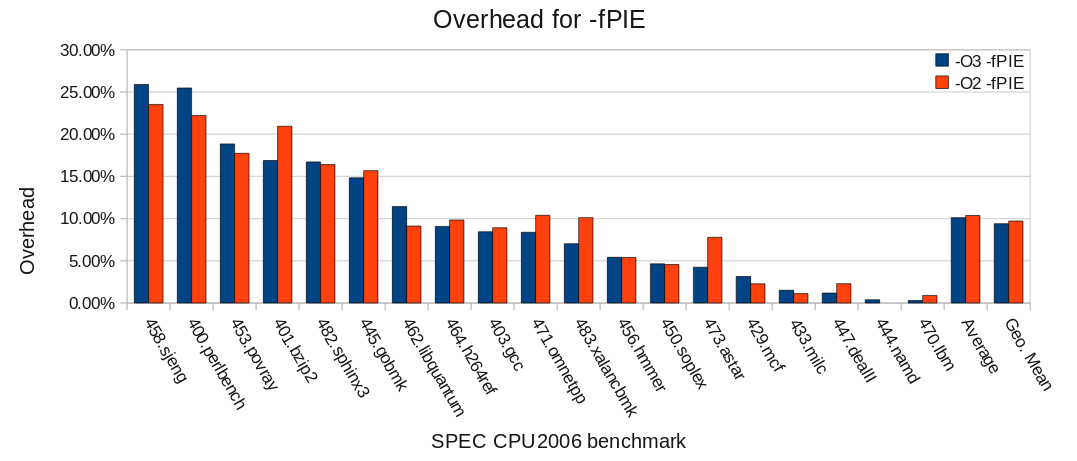
\includegraphics[width=\textwidth]{../mitigate/pie-cost}
\imagecredit{Payer, ``Too much PIE is bad for performance'', ETH Zurich Tech Report}
\end{frame}

\begin{frame}{position independence cost: Linux}
\begin{itemize}
    \item geometric mean of SPECcpu2006 benchmarks on x86 Linux
        \begin{itemize}
            \item with particular version of GCC, etc., etc.
        \end{itemize}
    \item 64-bit: 2-3\% (???)
        \begin{itemize}
        \item ``preliminary result''; couldn't find reliable published data
        \end{itemize}
    \item 32-bit: 9-10\%
    \item depends on compiler, \ldots
\end{itemize}
\end{frame}

\begin{frame}{position independence: deployment}
\begin{itemize}
    \item common for a very long time in dynamic libraries
    \item default for all executables in\ldots
    \vspace{.5cm}
    \item Microsoft Visual Studio 2010 and later
        \begin{itemize}
        \item \texttt{DYNAMICBASE} linker option
        \end{itemize}
    \item OS since 10.7 (2011)
    \item Fedora 23 (2015) and Red Hat Enterprise Linux 8 (2019) and later
        \begin{itemize}
        \item default for ``sensitive'' programs earlier
        \end{itemize}
    \item Ubuntu 16.10 (2016) and later (for 64-bit), 17.10 (2017) and later (for 32-bit)
        \begin{itemize}
        \item default for ``sensitive'' programs earlier
        \end{itemize}
\end{itemize}
\end{frame}



\section{backup slides}
\begin{frame}{backup slides}
\end{frame}


\begin{frame}[fragile,label=reloc]{recall: relocation}
\lstset{
    language=myasm,
    style=small,
    moredelim={**[is][\btHL<1>]{~1~}{~end~}},
    moredelim={**[is][\btHL<2>]{~2~}{~end~}},
}
\begin{lstlisting}
.data
string: .asciz "Hello, World!"
.text
main:
    movq $~1~string~end~, %rdi /* NOT PC/RIP-relative mov */
\end{lstlisting}
    generates: (\texttt{objdump --disassemble --reloc})
\lstset{
    language={},
    style=small,
    moredelim={**[is][\btHL<1>]{~1~}{~end~}},
    moredelim={**[is][\btHL<2>]{~2~}{~end~}},
}
\begin{lstlisting}
   0:   48 c7 c7 00 00 00 00    mov    $0x0,%rdi
                        ~1~3: R_X86_64_32S .data~end~
\end{lstlisting}
    \begin{itemize}
        \item \myemph{relocation record} says how to fix \texttt{0x0} in \texttt{mov}
            \begin{itemize}
                \item 3: location in machine code
                \item \texttt{R\_X86\_64\_32S}: 32-bit signed integer
                \item \texttt{.data}: address to insert
            \end{itemize}
    \end{itemize}
\end{frame}



\end{document}
